\clearpage
\section{Anonymization}
\label{sec:anonymization}
Anonymization of personal data refers to the process of removing personally identifiable information (PII) from data sets so that the individuals represented in the data cannot be identified. This is accomplished by either completely removing or replacing identifiable data with generic values. The purpose of anonymization is to protect the privacy of individuals while still allowing the data to be used for legitimate purposes. \\
Most of the recent implementations of anonymization work by masking the personal information of a person, such as names and surnames, telephone numbers, addresses, credit card numbers and so on. \\
One of the most famous libraries for anonymization is Presidio, developed by Microsoft. Presidio exploits pattern recognition with regex and Named Entity Recognition to find all the personal information and mask them. \\
The main disadvantage of such techniques is that often the personal subject can be identified through the so-called quasi-identifiers, that more often than not are not masked.
\\Here reported some examples that are not masked by Presidio:\\ \\
Original sentence
\begin{adjustwidth}{1cm}{}
    The new intern at my office, the one with red hair, caught covid last week 
\end{adjustwidth}
Sentence redacted by Presidio
\begin{adjustwidth}{1cm}{}
    The new intern at my office, the one with red hair, caught covid \textless DATE\_TIME \textgreater
\end{adjustwidth}
Original sentence
\begin{adjustwidth}{1cm}{}
    The boss of the HR department has made some weird comments about how I dress
\end{adjustwidth}
Sentence redacted by Presidio
\begin{adjustwidth}{1cm}{}
    The boss of the HR department has made some weird comments about how I dress 
\end{adjustwidth}
Our new approach exploits a Sequence to Sequence model called T5, which stays for Text-To-Text Transfer Transformer\todo{that stays for Text-To-Text Transfer Transformer}.
T5 is a model released by Google in 2019, it is a standard encoder-decoder transformer that, unlike BERT, always returns strings as outputs. This is why it is called a sequence-to-sequence model. \\
T5 is a unified model that can be applied for many downstream tasks, such as sentiment analysis, sentence completion, question answering\dots\\
In T5 architecture there are \textit{adapted layers} after each feed-forward layer, whose scope is to diminish the number of parameter updates for each fine-tuned model. In fact, \textit{adapted layers} are dense-ReLU-dense blocks that are designed so that their input dimensionality and output dimensionality are equal. This lets us insert them into the Transformer architecture without other changes. When fine-tuning for each different task, only the \textit{adapted layers} and the normalization layers will be updated. This results in a considerable reduction of parameter updates.\\
We followed a few-shot learning approach with T5. Rather than relying on a large amount of training data to allow a pre-trained model to adjust to a given task accurately, few-shot learning employs the use of a few examples to direct the training of a machine learning model with very minimal data. \\
For each category of tickets, we wrote 10 examples of "anonymized" tickets, where we removed all personal information and information that could be retraced to the original writer, maintaining only information that could be useful for analysis purposes.
Here are a couple of examples:\\ \\
Original sentence:
\begin{adjustwidth}{1cm}{}
    Dear Sir/Madame, I cannot stand anymore this discrimination and prejudice against French people at work
\end{adjustwidth}
Anonymization used for few-shot learning:
\begin{adjustwidth}{1cm}{}
    The employee is filling a complaint for discrimination based on nationality 
\end{adjustwidth}
Original sentence:
\begin{adjustwidth}{1cm}{}
    Hello, my name is Zacaredas Pinilla and I work at Laguna-Franco Spain. I am having trouble finding accommodation in the Algeciras area so if you could help me with this matter it would be greatly appreciated
\end{adjustwidth}
Anonymization used for few-shot learning:
\begin{adjustwidth}{1cm}{}
    The employee is asking for help finding an accommodation
\end{adjustwidth}
\begin{figure}[h] 
    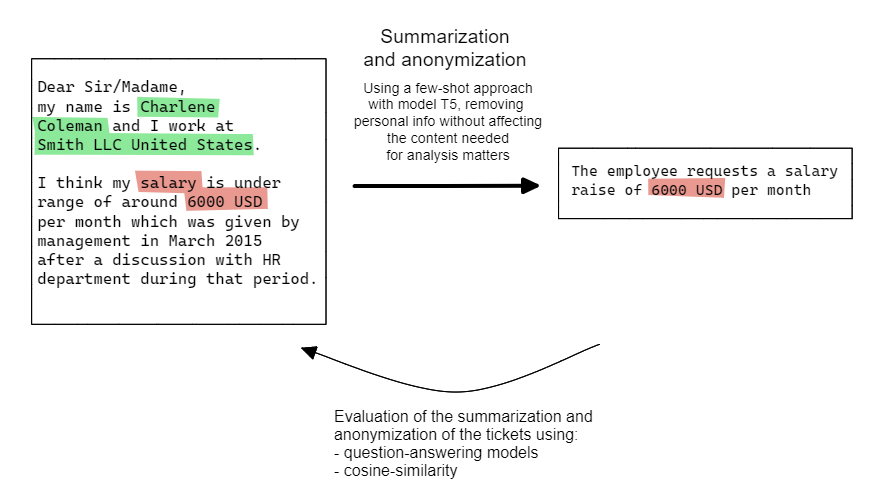
\includegraphics[width=\textwidth]{images/ticket_anonymization_schema.png}
    \caption{Schema of Ticket Anonymization}
    \label{fig:schema_ticket_anonymization}
\end{figure}    
To evaluate the goodness of anonymization and how much of the information has remained after the anonymization we have tested three different methods:
\begin{itemize}
    \item \textbf{QAGS}: Questions Answering and Generation for summarization
    \item \textbf{SUMMAQA}: Unsupervised metric for reinforced summarization model 
    \item \textbf{Cosine Similarity}: Cosine similarity of embeddings
\end{itemize}  
These models were created originally to evaluate the goodness of a summarization, we have adapted them to be used for evaluating our anonymization. \\
The first two methods follow the same philosophy: they generate questions to ask both the original version and the anonymized version of the tickets, looking if the answers are coherent. We call them Questions and Answers models.
However, they have a few key differences: SummaQA does not create natural sentence questions but uses as questions the masked version of the sentences. Instead, QAGS creates natural language questions using a pre-trained model.
\subsection{QAGS}
QAGS is an automatic evaluation protocol that is based on the assumption that if we reply to questions considering as factual bases the summary and the source, we can determine if the summary/anonymization is consistent with its source by comparing the answers. \\
QAGS works like this:
\begin{algorithm}[h]
    \caption*{QAGS}
    \begin{algorithmic}[1]
      \State A BART\cite{lewis2019bart} model is fine-tuned for question generation: the model receives both the answers and the source article from the NewsQA dataset and is trained to maximize the likelihood of the paired question
      \State At test time, named entities and noun phrases are extracted from the context using spaCy and are considered as answers candidates. The summary is used as the context.
      \State The BART model generates questions based on the summary and its entities
      \State A BERT model is fine-tuned for Question Answering on the SQuAD dataset
      \State We answer with the help of the fine-tuned BERT model the questions generated beforehand using both the source article and the summary to get two sets of answers. 
      \State We compare the corresponding answers using an answer similarity metric, and we get a final score averaging the answer similarity metric (f1 score) over all questions
    \end{algorithmic}
\end{algorithm}
\begin{figure}[h] 
    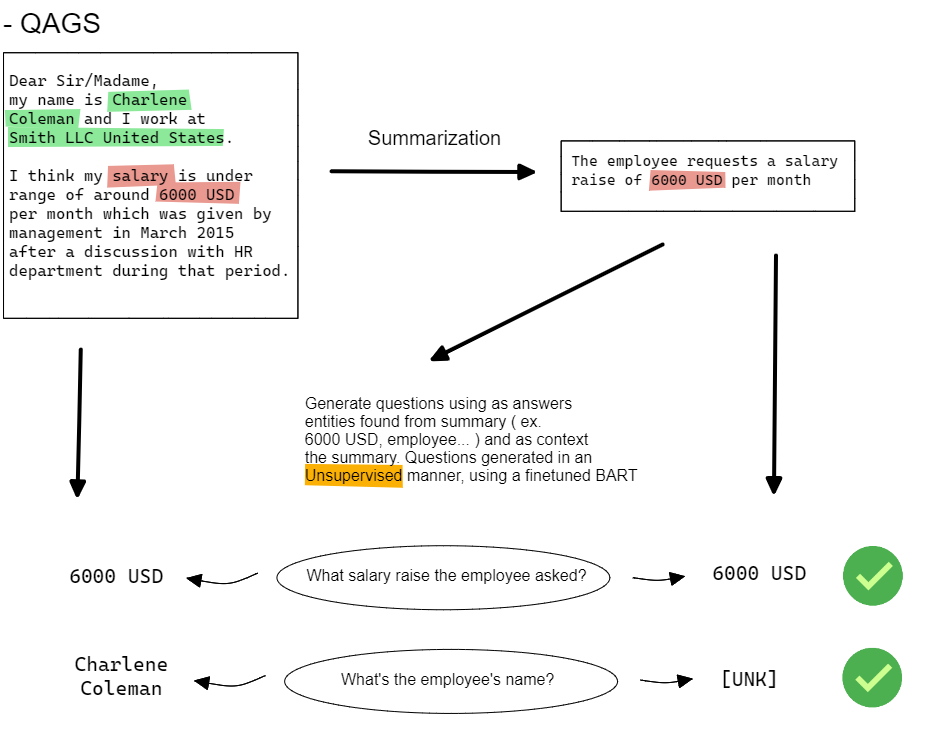
\includegraphics[width=\textwidth]{images/qa_models_qags.png}
    \caption{Schema of QAGS}
    \label{fig:schema_qags}
\end{figure}    
\newpage
\subsection{SUMMAQA}
SUMMAQA works similarly to QAGS, the main difference is that there is not a generative model to create the questions, in particular:
\begin{algorithm}[h]
    \caption*{SUMMAQA}
    \begin{algorithmic}[1]
      \State We find all the entities in the source text (the original ticket) with Spacy
      \State Create one sentence (which will be our question) for each entity. We keep only the sentence in which the entity is if there are more sentences. The entity will be masked. Ex: "Yesterday I went to Paris" becomes "Yesterday I went to [MASK]"
      \State The MASKED entities will be the True labels when calculating the metrics
      \State We answer the questions generated before using a fine-tuned version of BERT model, using both the source and the summarization/anonymization as contexts
      \State We compare the answers and calculate the f1 score for both contexts
    \end{algorithmic}
\end{algorithm}
\begin{figure}[h] 
    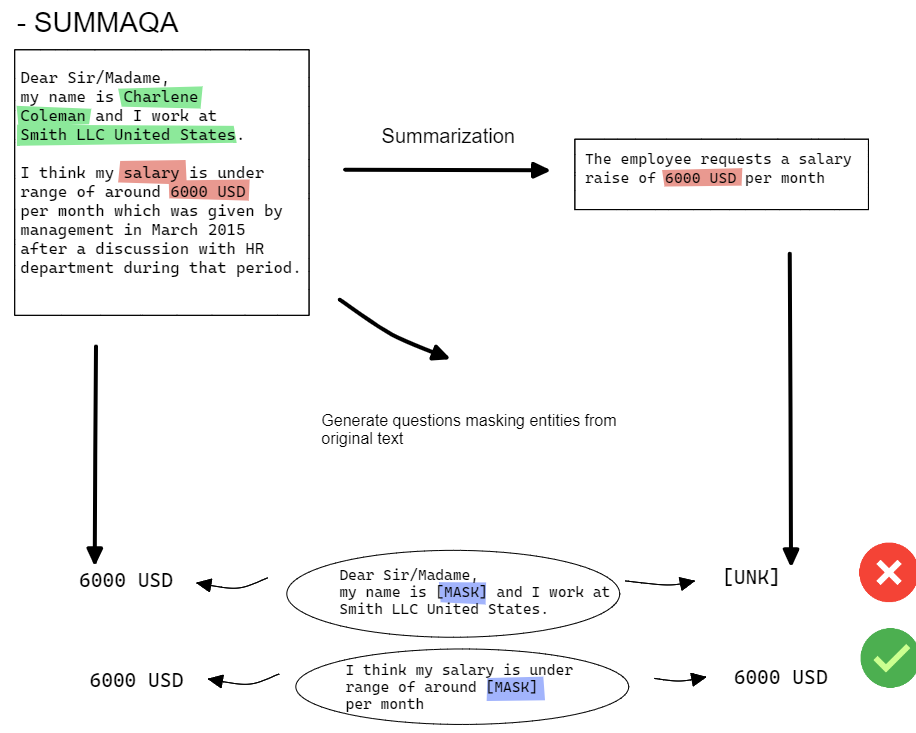
\includegraphics[width=\textwidth]{images/qa_models_summaqa.png}
    \caption{Schema of SUMMAQA}
    \label{fig:schema_summa_qa}
\end{figure} 
\newpage   
\subsection{Cosine Similarity}
We measured the cosine similarity between sentence embeddings of original text and summarization. The sentence embeddings used were calculated using Sentence-BERT, a modified version of the pretrained BERT network that uses siamese networks to obtain more meaningful embedding of the sentence, compared to getting the embedding of the [CLS] token or to average all the other embeddings.
\begin{figure}[h] 
    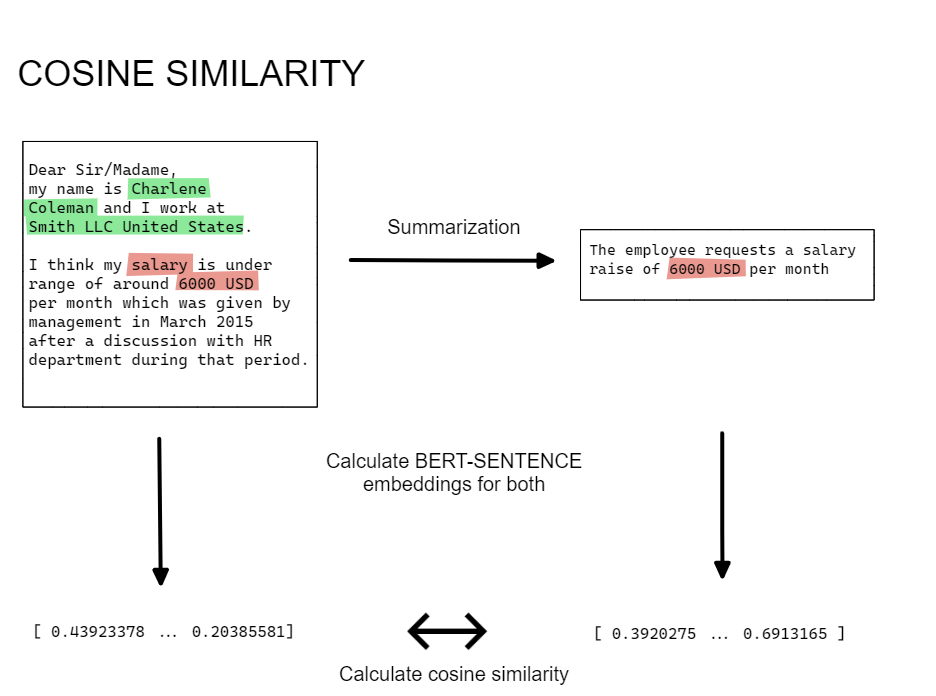
\includegraphics[width=\textwidth]{images/cosine_similarity.png}
    \caption{Schema of Cosine Similarity for }
    \label{fig:schema_cosine_similarity}
\end{figure}    
\subsection*{Result}
After testing all of the three methods described before, the one chosen was QAGS. The main reason why is its flexibility. Right now it was not implemented, but in future works it could be possible to add to the questions automatically generated by BART some questions written by the users to check whether a piece of information has been anonymized or not. \\
However, the numeric results are difficult to interpret, because sometimes we want to retain some information from the original text and sometimes we would prefer the information to be removed. 
%TODO: maybe put little schema of Siamese network of sentence-bert



